\documentclass{aamas2012}
% Setting letter size with pdflatex
\pdfpagewidth=8.5truein
\pdfpageheight=11truein

\usepackage{float}
\usepackage{makeidx}
\usepackage{amsmath}   
\usepackage{amsfonts}   
\usepackage[retainorgcmds]{IEEEtrantools}
\usepackage{thumbpdf}
\usepackage{multicol}   
\usepackage{graphicx}   
\usepackage{listings}
\usepackage{algorithm}
\usepackage{algorithmic}
\usepackage{tikz}
\usepackage{subfigure}

\usepackage{hyperref}
\hypersetup{ 
  pdftitle          = {Learning in a Small World},
  pdfauthor         = {Arun Tejasvi Chaganty, Prateek Gaur, Balaraman Ravindran},
  colorlinks        = true,
  linkcolor         = red,
  urlcolor          = red,
  citecolor         = blue,
}

% Section References
\newcommand{\secref}[1] {\hyperref[#1]{Section~\ref*{#1}}}
\newcommand{\eqnref}[1] {Equation \eqref{#1}}
\newcommand{\thmref}[1] {Theorem \ref{#1}}
\newcommand{\lmref}[1] {Lemma \ref{#1}}
\newcommand{\algoref}[1] {\hyperref[#1]{Algorithm~\ref*{#1}}}
%\renewcommand{\algorithmiccomment}[1]{\textit{// #1}}
%\theoremstyle{plain} \newtheorem{thm}{Theorem}

%Math Operators
\DeclareMathOperator {\argmax} {argmax}
\DeclareMathOperator {\sgn} {sgn}
\DeclareMathOperator {\trace} {tr}
\DeclareMathOperator{\E} {E}
\DeclareMathOperator{\Var} {Var}

\renewcommand{\Re} {\mathbb{R}}

\newcommand{\ud}{\, \mathrm{d}}
\newcommand{\diff}[1] {\frac{\partial}{\, \partial #1}}
\newcommand{\diffn}[2] {\frac{\partial^{#2}}{\, \partial {#1}^{#2}}}
\newcommand{\tuple}[1] {\langle #1 \rangle}

%Short hand
\newcommand{\mdp} {\ensuremath{\mathcal{M}}}
\newcommand{\states} {\mathcal{S}}
\newcommand{\actions} {\mathcal{A}}
\newcommand{\transitions} {\mathcal{P}}
\newcommand{\rewards} {\mathcal{R}}
\newcommand{\graph} {\mathcal{G}}
\newcommand{\policy} {\pi}
\newcommand{\initset} {\mathcal{I}}
\newcommand{\stopcond} {\beta}
\newcommand{\option} {\tuple{ \initset,\policy,\stopcond} }
\newcommand{\options} {\mathcal{O}}

%Math Operators
\DeclareMathOperator {\ball} {B}
\DeclareMathOperator {\ballf} {B^{f}}
\DeclareMathOperator {\sball} {b}
\DeclareMathOperator {\sballf} {b^{f}}

%Short hand
\newcommand{\arbcnst} {\tilde{c}}
\newcommand{\greedyalgo} {\ensuremath{\mathcal{GA}~}}

\newtheorem{theorem}{Theorem}
\newtheorem{lemma}{Lemma}
\newdef{definition}{Definition}
\newdef{example}{Example}
\newcommand{\draft}[1]{\textbf{TODO: #1}}

\title{Learning in a Small World}

% Author information
\numberofauthors{3}
\author{ 
\alignauthor 
Paper  280
% Commented until we get accepted
% Arun Tejasvi Chaganty\\
%        \affaddr{Deptt. of Computer Science and Engineering,}\\
%        \affaddr{IIT Madras}\\
%        \affaddr{Chennai, India - 600036}\\
%        \email{arunc@cse.iitm.ac.in}
% \alignauthor
% Prateek Gaur\\
%        \affaddr{Deptt. of Computer Science and Engineering,}\\
%        \affaddr{IIT Madras}\\
%        \affaddr{Chennai, India - 600036}\\
%        \email{prtkgaur@cse.iitm.ac.in}
% \alignauthor
% Balaraman Ravindran\\
%        \affaddr{Deptt. of Computer Science and Engineering,}\\
%        \affaddr{IIT Madras}\\
%        \affaddr{Chennai, India - 600036}\\
%        \email{ravi@cse.iitm.ac.in}
} 

\begin{document}

\maketitle
%\pagebreak

% Outline
\begin{abstract}

Understanding how we are able to perform a diverse set of complex tasks
has been a central question for the Artificial Intelligence community.
One popular approach is to use temporal abstraction as a framework to
capture the notion of subtasks. However, this transfers the problem to
finding the right subtasks, which is still an open problem. Existing
approaches for subtask generation require too much knowledge of the
environment, and the abstractions they create can overwhelm the agent.
We propose a simple algorithm inspired by small world networks to learn
subtasks while solving a task that requires virtually no information of
the environment. Additionally, we show that the subtasks we learn can be
easily composed by the agent to solve any other task; more formally, we
prove that any task can be solved using only a logarithmic combination
of these subtasks and primitive actions. Experimental results show that
the subtasks we generate outperform other popular subtask generation
schemes on standard domains. 

%\draft{What is our contribution?}
% Relevance to lifelong learning?

\end{abstract}


\category{I.2.6}{Artificial Intelligence}{Learning}
\category{I.2.8}{Artificial Intelligence}{Problem Solving, Control Methods and Search}
\terms{Algorithms, Theory, Experimentation}
\keywords{reinforcement learning, options framework, social network analysis, small world phenomenon}

% Introduction: Motivate the problem (using lifelong learning,
% transfer)
% Emphasise on not blowing up state space, summarise results
\section{Introduction}
\label{sec:intro}

% General Introduction
In large domains, RL agents generally require a large number of samples to learn
a good policy. The options framework proposed by Sutton, Precup and Singh
\cite{SuttonPrecupSingh1998} provides extended actions for which a policy is
already learnt, reducing the complexity of the learning task, and generally
making the learning task faster.  An open question in the options framework is
discovering the options themselves.  There has been substantial work to learn
options, mainly focussed around identifying ``bottleneck'' states, either
empirically as in the work bye Stolle \cite{Stolle}, or more recently, using
graph theoretic methods like betweeness \cite{Simsek} or graph partitions
\cite{Simsek2005} explored by Simsek and Barto.

% Motivation
In this work, we propose a method for creating options motivated from a
cognitive perspective, based on the following hypothesis: we memorise many
actions, not necessarily bottleneck ones, and evolve them. Based on their
necessity in solving problems these actions are either reinforced, or gradually
forgotten. The actions could be of varying complexity, and it is intuitive to
expect that we probably learn a great deal more {\em simple} actions than
complex ones. In context of the options framework, these actions correspond to
options, and ``complex actions'' correspond to longer options.

% Our options
A desirable set of options gives the agent a set of skills which can be put
together to efficiently accomplish almost any task. From the perspective of the
state-space interaction graph, this is similar to the problem of distributed
search studied by Kleinberg \cite{Kleinberg}; adding edges to a graph such that
any node can be efficiently reached. Guided by this intuition, the method we
propose generates options using a generalisation of the inverse-square law,
along the lines of the small-world graph generation model proposed by Kleinberg.

% Summary of the results
Our results show that agents trained using our `small-world' options indeed
perform well, and converge to optimal performance quickly and with little
variance. 


% Background: Define MDPs, Options
\section{Background}
\label{sec:background}

% MDPs
In reinforcement learning, the standard representation of an environment
and task instance is a Markov decision process (MDP). An MDP can be
represented as the tuple, \\ $\tuple{ \states, \actions, \transitions,
\rewards, \gamma }$, where $\states$ and $\actions$ are finite sets of
states and actions, $\transitions: \states \times \actions \times
\states \to [0,1]$ describes the dynamics of the world through
state-action transition probabilites, $\rewards: \states \times \actions
\to \Re$ describes the task at hand by ascribing rewards for state
transitions, and $\gamma \in [0,1]$ is a discount factor that weighs the
value of future rewards.

In this setting, an agent in a state $s \in \states$ chooses an action
$a \in \actions$, and moves to a state $s'$ with probability
$\transitions(s,a,s')$, receiving a reward $\rewards(s,s')$. The
objective of the agent is to find a policy $\pi: \states \times \actions
\to [0,1]$, i.e. a decision procedure for selecting actions, that
maximises the reward it accumulates in the long run, $R = \sum_{i}
\gamma^i r_i$. $R$ is also called the return.

We define the value function $V: \states \to \Re$ to be the expected
return from $s$, and $Q: \states \times \actions \to \Re$ to be the
expected return from $s$, after taking the action $a$. The optimal value
function must satisfy the Bellman optimality equation, 
\begin{eqnarray*}
  V(s) &=& \max_{a} \rewards(s,a) + \gamma \sum_{s' \in \states} \transitions(s,a,s') V(s') \\
  Q(s,a) &=& \rewards(s,a) + \gamma \sum_{s' \in \states} \transitions(s,a,s') \max_{a'} Q(s',a').
\end{eqnarray*}

Given an optimal $Q$, an agent can construct an optimal policy,
$\pi(s,a^*) = 1$ when $a^* = \argmax_{a} Q(s,a)$, and $0$ otherwise. In
principle, if the agent knew the MDP, it could construct the optimal
value function, and from it an optimal policy.  However, in the usual
setting, the agent is only aware of the state-action space, $\states$
and $\actions$, and must learn $Q$ through exploration. The Q-learning
algorithm learns $Q$ with a simple update for every step the agent
takes, 
\begin{eqnarray*}
    Q(s,a) &=& Q(s,a) + \alpha [ r + \gamma \max_{a'} Q(s',a') - Q(s,a) ],
\end{eqnarray*}
\noindent
where $\alpha \in [0,1]$ is a parameter that controls the learning rate.
It has been shown that the Q-learning algorithm converges to the optimal
value function in the limit with fairly permissive assumptions.

% Options
The options framework provide a temporal abstraction for subtasks. An
option $\option$ is described by an initiation set $\initset \subset
\states$, a policy $\pi$, and a terminating condition $\beta$.  An agent
can exercise an option in any state $s \in \initset$, following which,
it will follow the policy $\pi$ described by the option, until the
terminating condition $\beta(s)$ is satisfied. The terminating condition
$\beta$ can be stochastic.

Several learning algorithms have been proposed for agents using options
\cite{SuttonPrecupSingh1999,BartoMahadevan2003}. One simple such method that
we will use is MacroQ, a generalisation of the Q-learning algorithm
described above. The MacroQ algorithm updates the value function only
after completion of the option. If the option $o$ was initiated in the
state $s$, and continues for $k$ steps before terminating in $s'$, the
corresponding $Q$ function update will be,
\begin{eqnarray*}
    Q(s,o) &=& Q(s,o) + \alpha [ r + \gamma^{k} \max_{o' \in \actions \cup \options} Q(s',o') - Q(s,o) ].
\end{eqnarray*}

Different tasks in the same domain can be described by different
$\rewards$. Let $\rewards$ be sampled from the family $\Rewards$. Our
objective then is to find a set of options $O$ that reduces the expected
learning time over $\Rewards$.

\begin{example}
  \label{example:taxi}

\begin{figure}[th]
    \centering
    \documentclass{article}
\usepackage{standalone}
\usepackage{tikz}
\usetikzlibrary{external}
\tikzexternalize % activate!

\begin{document}
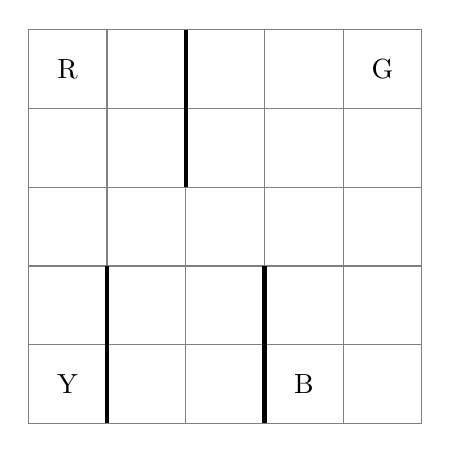
\begin{tikzpicture}
    % Grid
    \draw[step=1,color=gray] (0,0) grid (5,5);
    
    % Walls
    \draw[line width=1.5pt] (2,5) -- (2,3);
    \draw[line width=1.5pt] (1,0) -- (1,2);
    \draw[line width=1.5pt] (3,0) -- (3,2);

    % Pads
    \draw (0.5,4.5) node {R};
    \draw (0.5,0.5) node {Y};
    \draw (3.5,0.5) node {B};
    \draw (4.5,4.5) node {G};
\end{tikzpicture}
\end{document}

    \label{fig:taxi-domain}
    \caption{The Taxi Domain}
\end{figure}
To make the discussion more tangible, let us look at an example, the
Taxi domain, shown in \figref{fig:taxi-domain}. The agent is a taxi
navigating in this road-map. It must pick up a passenger at one of the
4 pads, R, G, B or Y.  Subsequently, it must carry the passenger to a
destination, which is also one of the above four pads. The states of
the taxi would then be a tuple containing the location of the
passenger (in one of the four pads, or within the taxi), the
destination of the passenger, and location of the taxi in the map.
The actions the taxi can perform are moving up, down, left or right in
the map, as well as pick up or drop a passenger at a pad. 
Typical options for such a domain would be an option that can be
started anywhere, and has a policy that takes the taxi to the one of
the pads in the shortest possible manner. Such an option is generic,
and does not depend on where the passenger or destination are. The RL
agent must then learn to choose the right option when picking up the
passenger.
\end{example}


% Define the algorithm. Prove the interesting result
\section{Approach}
\label{sec:approach}

% MDPs
Before we describe our approach for generating options, we briefly review Markov
Decision Processes (MDPs) and options framework. An MDP $\tuple{
    \states,\actions,\rewards }$ is a standard representation for a RL problem,
where $\states$ is the set of states in the world, $\actions$ is the set of
actions that take the agent from one state to another with some transition
probability, and $rewards$ is the set of rewards obtained when moving from one
state to another. The objective is to find a decision procedure or policy $\pi$
that maximises the return, or the rewards accumulated in the long run. 

% Options
An option $\option$ is described by an initiation set $\initset \subset
\states$, a policy $\pi$, and a terminating condition $\beta$. An agent can
exercise an option in any state $s \in \initset$, following which, it will
follow the policy $\pi$ described by the option, until the terminating condition
$\beta(s)$ is satisfied. The terminating condition $\beta$ can be stochastic as
well. 

% Example

\begin{figure}[h]
    \center
    \documentclass{article}
\usepackage{standalone}
\usepackage{tikz}
\usetikzlibrary{external}
\tikzexternalize % activate!

\begin{document}
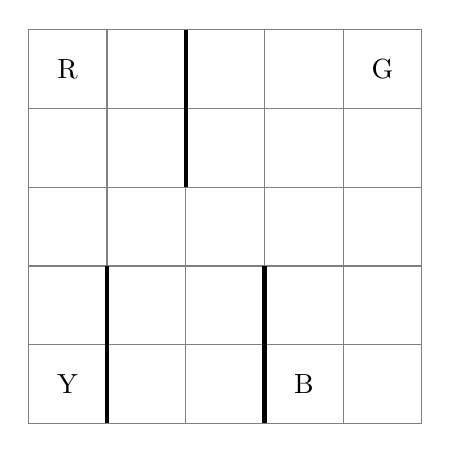
\begin{tikzpicture}
    % Grid
    \draw[step=1,color=gray] (0,0) grid (5,5);
    
    % Walls
    \draw[line width=1.5pt] (2,5) -- (2,3);
    \draw[line width=1.5pt] (1,0) -- (1,2);
    \draw[line width=1.5pt] (3,0) -- (3,2);

    % Pads
    \draw (0.5,4.5) node {R};
    \draw (0.5,0.5) node {Y};
    \draw (3.5,0.5) node {B};
    \draw (4.5,4.5) node {G};
\end{tikzpicture}
\end{document}

    \caption{The Taxi Domain}
    \label{fig:taxi-domain}
\end{figure}

To make the discussion more tangible, let us look at an example, the Taxi
domain, shown in \autoref{fig:taxi-domain}. The agent is a taxi navigating in
this road-map. It must pick up a passenger at one of the 4 pads, A, B, C or D.
Subsequently, it must carry the passenger to a destination, which is also one of
the above four pads. The states of the taxi would then be the location of the
passenger (in one of the four pads, or within the taxi), the destination of the
passenger, and location of the taxi in the map. The actions the taxi can perform
are moving up, down, left or right in the map, as well as pick up a passenger or
drop him at the destination.  Typical options for such a domain would be an
option that can be started anywhere, and has a policy that takes the taxi to the
one of the pads in the shortest possible manner. Such an option is generic, and
does not depend on where the passenger or destination are. The RL agent must
then learn to choose the right option when picking up the passenger.

\begin{figure}[h]
    \center
    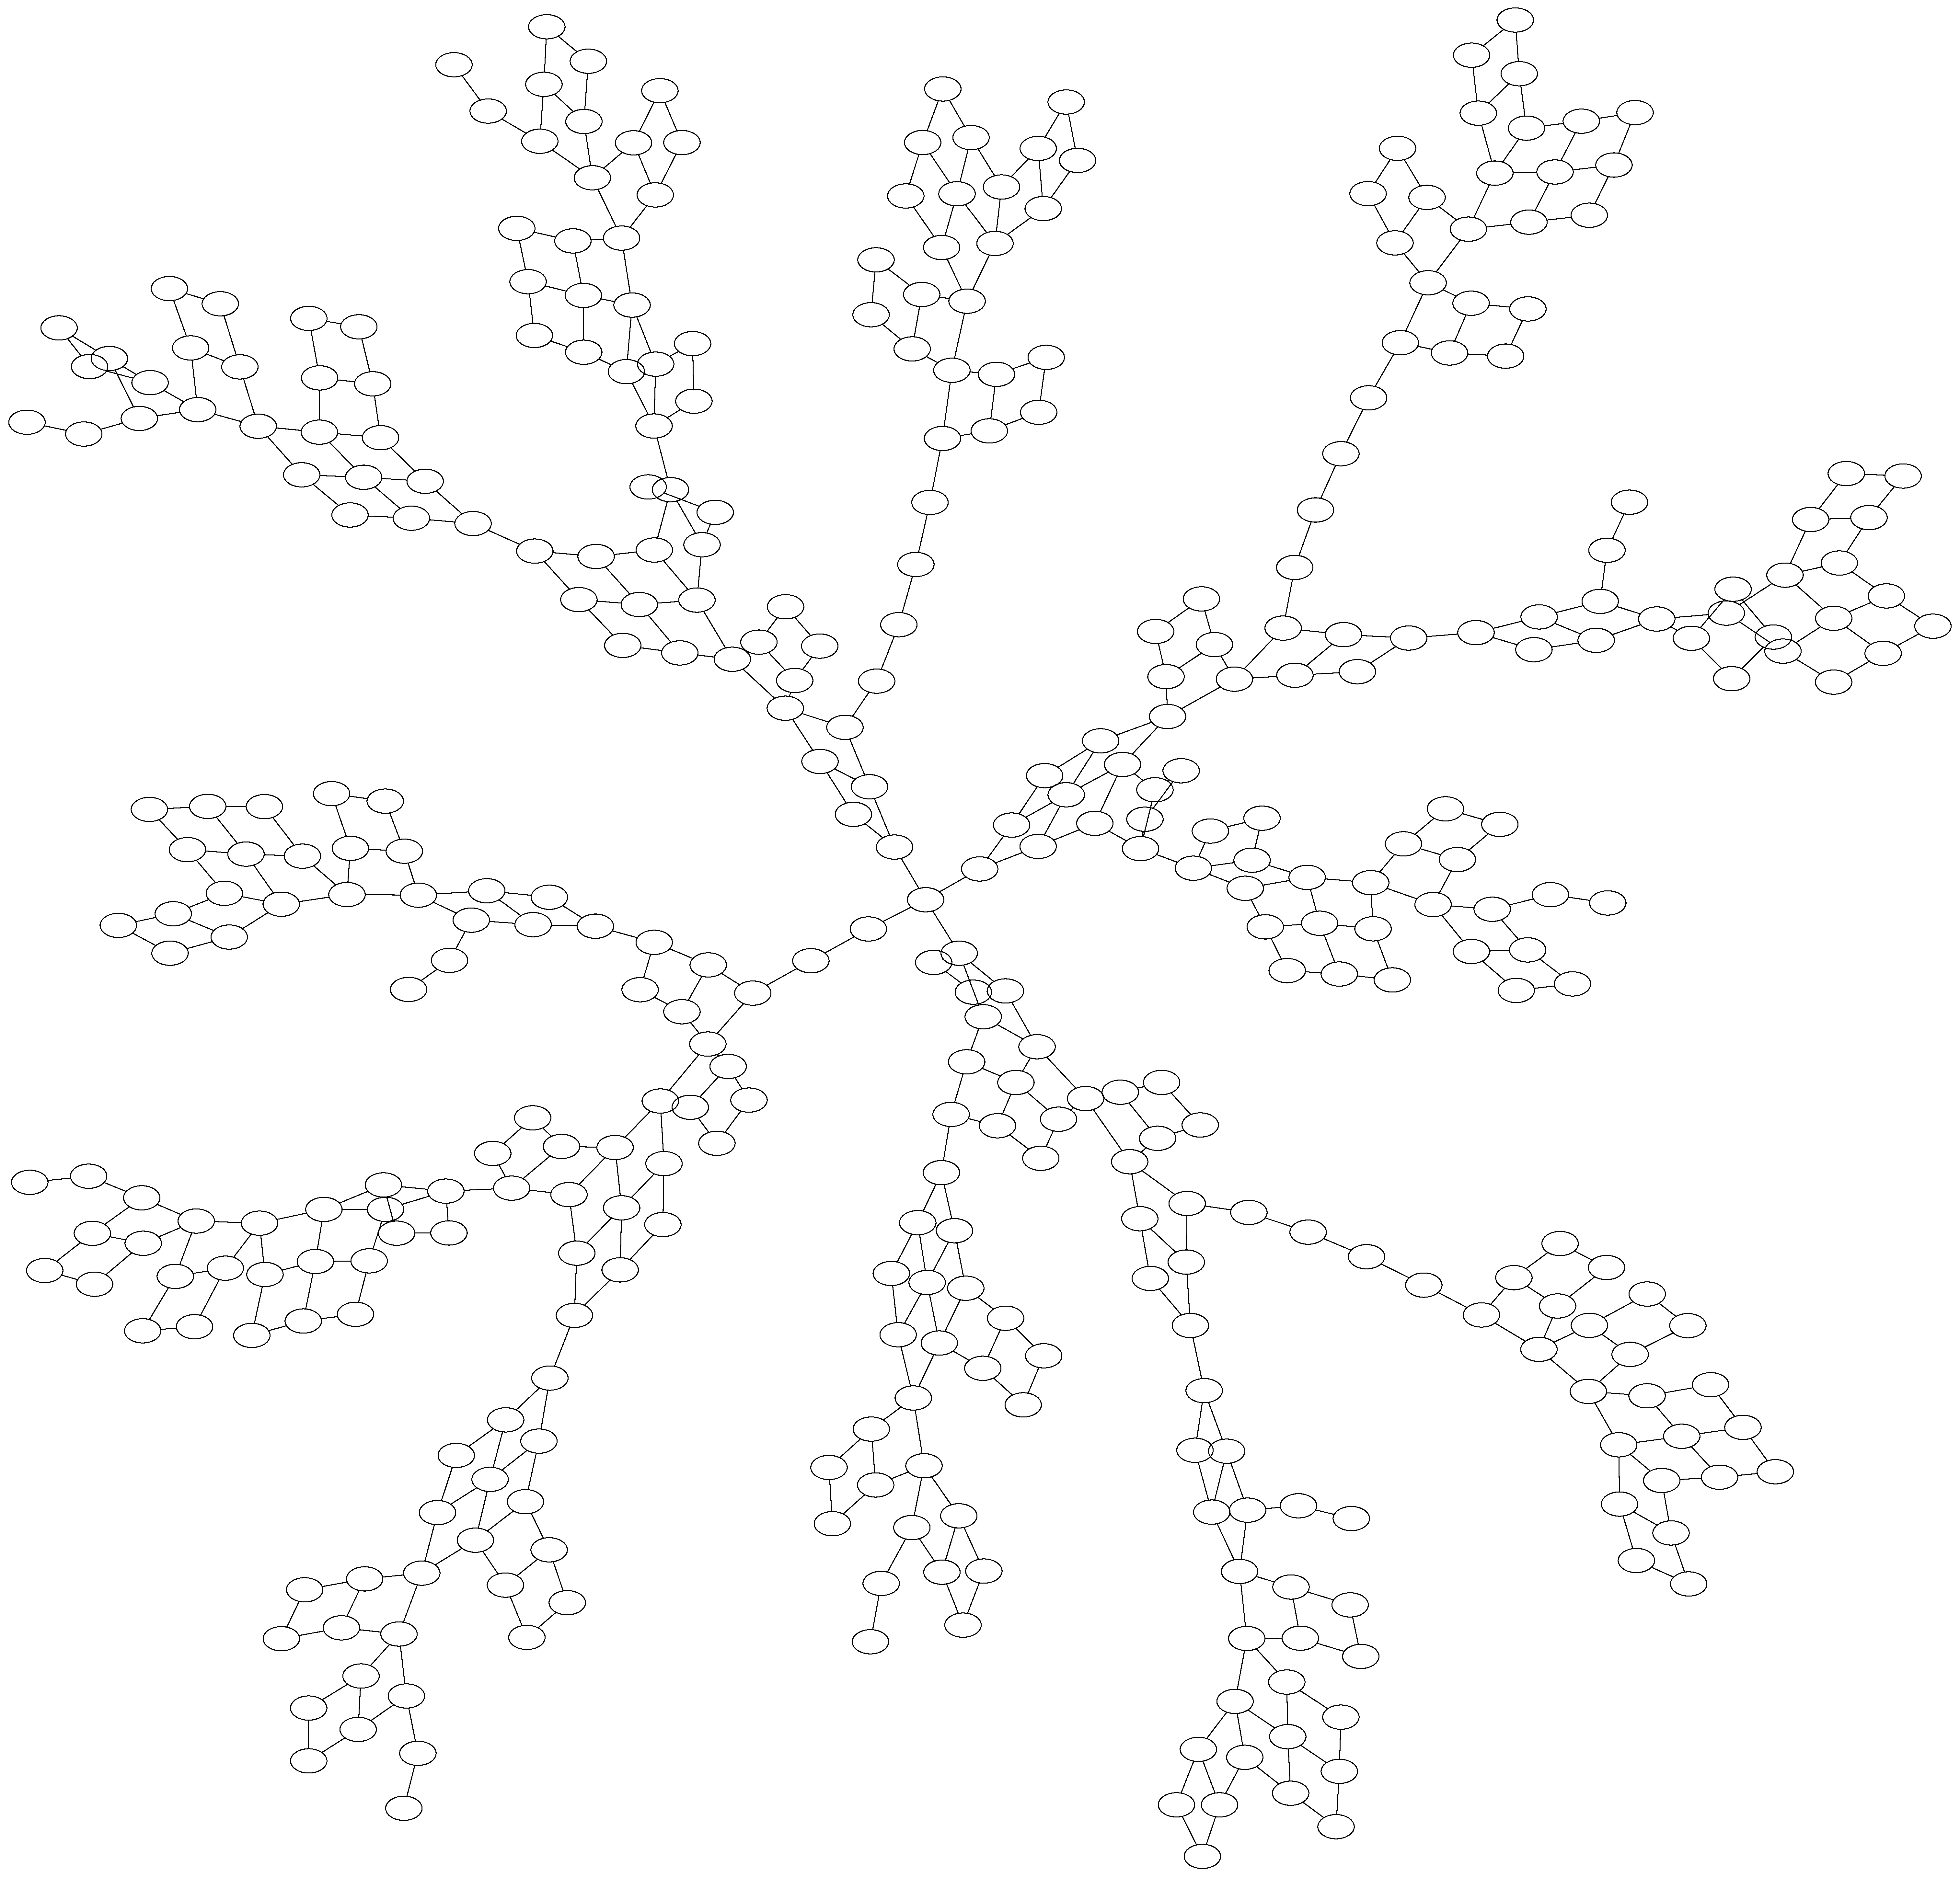
\includegraphics[width=3in]{figures/taxi1}
    \caption{State Space Graph for the Taxi Domain}
    \label{fig:taxi-graph}
\end{figure}

% Graph-based
It is easy to construct a graph $\graph$ out of the state-space described by an
MDP. The states $\states$ become the nodes of the graph, and $\actions$ become
the edges, with the transition probabilites serving as the weights. The edges
are also attributed with the rewards described by $\rewards$. Options can be
viewed to be paths along the graph. The Taxi domain just defined translates to
a graph shown in \autoref{fig:taxi-graph}.

% Constructing Options 
We construct an option `short-circuiting' two states using a policy constructed
from the shortest path on this graph. For every state $x$, we select a state to
be short-circuited $y$ with using a multinomial distribution with weight
proportional to the distance between them in the state space, i.e. $w(x,y)
    \propto d(x,y)^{-r}$. 

Another example of constructing an option on this graph would be to define a
policy that takes any state to a particular one along the shortest path. This is
the approach adopted by Simsek and Barto in \cite{Simsek}, where local maxima of
the betweenness scores are used to identify bottlenecks, and options defined to
reach these bottlenecks optimally from any state.

% Describe Macro-Q and Intra-Option-Q
Several learning algorithms have been proposed for agents using options
\cite{SuttonPrecupSingh1998,BartoMahadevan}. A simple such method is Macro
Q-learning, a generalisation of the Q-learning methods. The MacroQ algorithm
updates the value function only after completion of the option. If the option
$o$ was initiated in the state $s$, and continue for $k$ steps before
terminating in $s'$, the corresponding back-up will be,

\begin{IEEEeqnarray*}{rCl}
    Q(s,o) &=& Q(s,o) + \alpha [ r + \gamma^{k} \max_{o' \in \options_{s'} \cup \actions_{s'}} Q(s',o') - Q(s,o) ].
\end{IEEEeqnarray*}

Another method, Intra-option Q-learning, exploits the experience gathered during
the trajectory, instead of only at the end of it. In this approach, every step
from $s$ to $s'$ using $a \in \actions$ is used to back up the value function of
every option $o \in \options$ which can be used in $s$, and whose policy has a
non-zero probability of using the action $a$ using the following update,

\begin{IEEEeqnarray*}{rCl}
    Q(s,o) &=& Q(s,o) + \alpha [ r + \gamma Q(s',o) - Q(s,o) ].
\end{IEEEeqnarray*}
\noindent
The value-function for every action along the trajectory is also updated, using
the usual Q-learning backups.

% \begin{IEEEeqnarray*}{rCl}
%     x &=& y \\
%       &=& z \\
% \end{IEEEeqnarray*}

% \begin{figure}[s]
%     \centering
%     \includegraphics[width=5in]{filename}
%     \caption{ }
%     \label{fig:high-variance-rtt}
% \end{figure}

% Describe the algorithms to; a) generate small world options b)
% extract from learning episodes
\section{Options from Experience} 
\label{sec:algo}

In \secref{sec:theory}, we remarked that we need to generate $O(|S|)$
options. Given the scale of this number, we require an algorithm to
efficiently generate options within a budget of training epochs in order
for small world options to be practical. Drawing insight from the proof
of \thmref{thm:small-world}, the objective of small world options is to
bring the agent into an exponentially smaller neighbourhood of the
maximal value state. This suggests that cheaply generated options may
still be acceptable.

The algorithm (\algoref{algo:small-world-experience}) we propose takes
a given MDP $\mdp$, and trains an agent to learn $T$ different tasks
(i.e. different $\rewards$) on it, evenly dividing the epoch budget
amongst them. With each learned task, we certainly will have a good policy
for path options from any state to the state of maximal value, $M_v$.
However, we observe that will also have a good policy for path options
from $u$ to $v$ is the path is `along the gradient' of $Q$, i.e. when
$V(u) < V(v) < V(M_v)$. Observing that $V(s) \approx \argmax_{v}
Q(s,\pi(s))$, we detail the algorithm to construct options from the
$Q$-value function in \algoref{algo:qoptions}. We use this algorithm to
construct many options from a single task solution.

\begin{algorithm}[H]
  \caption{Small World Options from Experience}
  \label{algo:small-world-experience}
  \begin{algorithmic}[1]
      \REQUIRE $\mdp$, $\Rewards$, $r$, $n$, epochs, $T$
      \STATE $O \gets \emptyset$
      \FOR{ $i= 0 \to T$ }
        \STATE $\rewards \sim \Rewards$
        \STATE $Q \gets $ Solve $\mdp$ with $\rewards$ using
            $\frac{\textrm{epochs}}{T}$ epochs
        \STATE $O' \gets $ QOptions( $Q$, $r$,
            $\frac{n}{T}$ )
        \STATE $O \gets O \cup O'$
      \ENDFOR
      \RETURN A random subset of $n$ options from $O$
  \end{algorithmic}
\end{algorithm}
\begin{algorithm}[H]
  \caption{{\bf QOptions}: Options from a $Q$-Value Function}
  \label{algo:qoptions}
  \begin{algorithmic}[1]
      \REQUIRE $Q$, $r$, $n$
      \STATE $O \gets \emptyset$
      \STATE $\pi \gets $ greedy policy from $Q$
      \FORALL{ $s$ in $\states$ }
        \STATE Choose an $s'$ according to $P_r$
        \IF{ $Q(s', \pi(s')) > Q(s, \pi(s))$ }
          \STATE $O \gets O \cup \tuple{\{s\}, \pi, \{s'\} \cup \{t \mid Q(s',\pi(s')) < Q(t, \pi(t))\} }$
        \ENDIF
      \ENDFOR{ $s$ in $\states$ }
      \RETURN A random subset of $n$ options from $O$
  \end{algorithmic}
\end{algorithm}

We note here except for sampling $s'$ from $P_r$, we do not require any
knowledge of the MDP, nor do we need to construct a local model of the
same. $s'$ can approximately be sampled using $\frac{E[l]}{\log(|S|)}$
in place of $P_r$. 


% Experiment section
%\section{Empirical Performance}
\label{sec:experiments}
% Experimental results

% Graphs
\begin{figure}[h]
\centering
\subfigure[$P_2$-Distributed Options]{
\includegraphics[height=2in]{figures/rooms-options}
\label{fig:rooms-options}
}
\subfigure[Cumulative Return]{
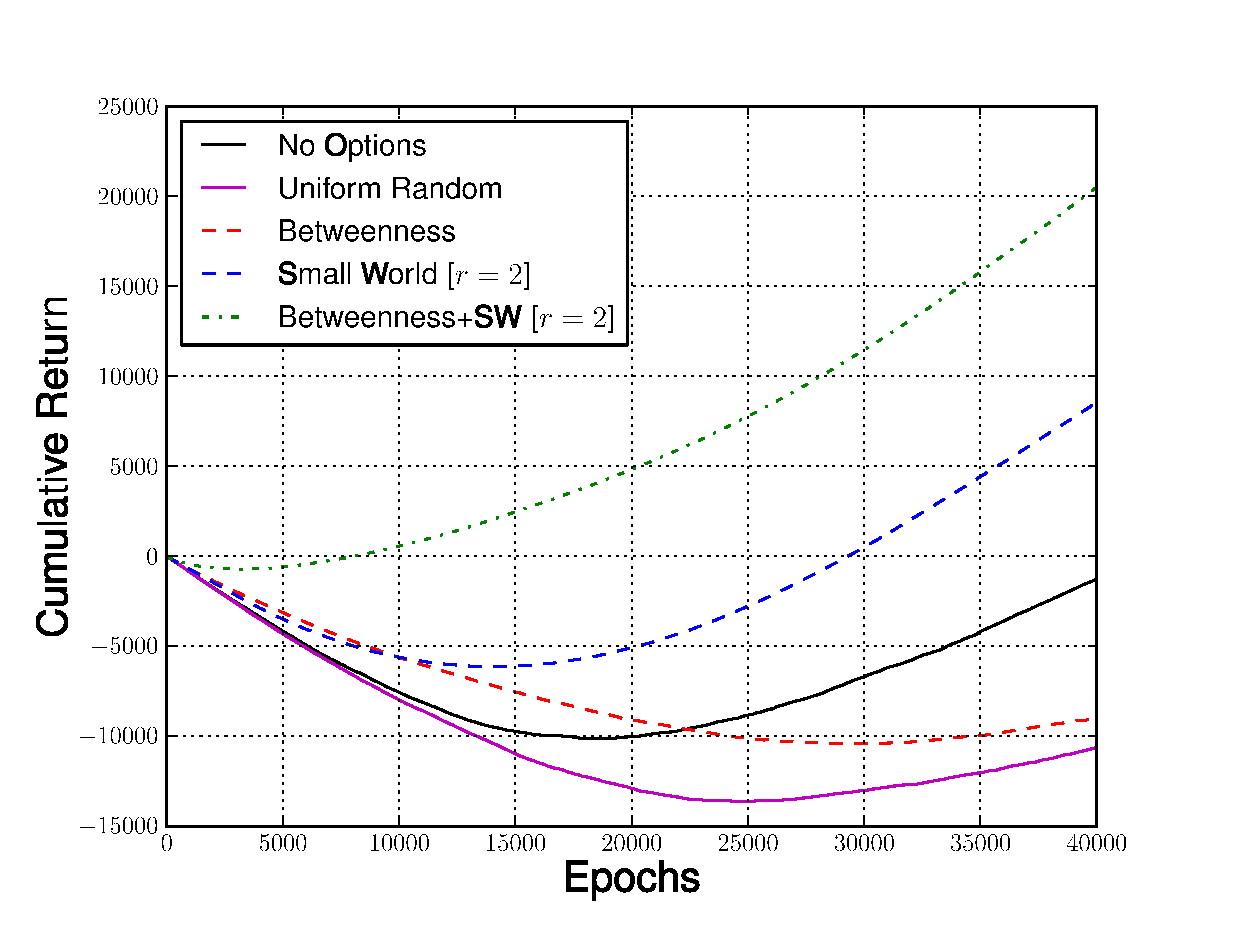
\includegraphics[height=2.2in]{figures/rooms-algos-200}
\label{fig:rooms-performance}
}
\label{fig:rooms}
\caption{Results on the Rooms Domain}
\end{figure}

% Brief description of Rooms, Taxi and Arbitrary Navigation domains.
We trained agents using the MacroQ algorithm, and tested it on three
standard domains, Taxi, Rooms and a $20\times20$ arbitrary navigation
task, and compared the performance of agents using options generated
(i) using betweenness centrality, (ii) using $P_0$ (uniformly random
paths), (iii) using paths between nodes selected using $P_{r>0}$, and
(iv) using a combination of (i) and (iii).  The performance of
$P_r$-distributed options was worst when $r=0$, and increased to peak
at a particular $r$ before decreasing again; behaviour also observed
in Kleinberg's work. With appropriate $r$, $P_r$-distributed options
accumulate significant return, and outperform bottleneck-based methods
on navigation tasks. 

% Observations
% When goal state and start state are further apart, the options that stand out
% are more


% Discuss conclusions
\section{Conclusions and Future Work}
\label{sec:conclusions}

% Contributions
% - new scheme for generating options
We have devised a new scheme to generate options based on small world
network model. The options generated satisfy an intuitive criteria, that
the subtasks learnt should be easily composed to solve any other task.
The options greatly improve the connectivity properties of the domain,
without leading to a state space blow up. Finally, they are interesting
from a theoretical perspective, as they require only a logarithmic
number of decisions required in a learning task.

% - absolutely model-free
Experiments run on standard domains show significantly faster learning
rates using small world options. At the same time, we have shown that
learning small world options can be cheaper than learning bottleneck
options, using a natural algorithm that extracts options from a handful
of tasks it has solved. Another advantage of the scheme is that is does
not require a model of the MDP. 

% Further work
% - dynamically add/remove options
% - figuring out r
As future work, we would like to characterise what the exponent $r$
should be in a general domain. Given the ease with which options can be
discovered, it would be interesting to experiment with a dynamic scheme
that adds options on the fly, while solving tasks.



\bibliographystyle{abbrv}
\bibliography{ref}{}

\balancecolumns

\appendix
\section{Small Worlds}
\label{sec:small-world-theory}

% Introduction and motivation for the proof
In this section we will tackle the proof of the main theorem in
\secref{sec:theory},

\begin{theorem}
  %
  Let $f : V \to \Re$ be a function embedded on the graph $\graph(V,E)$,
  such that, $\kappa_1 \|u-v\| - c_1 \le \|f(u) - f(v)\| \le \kappa_2
  \|u - v\| - c_2$, where $0 \le \kappa_1 \le \kappa_2$, and $0 \le c_2
  \le \frac{c_1}{2}$. Let $M_f$ be the global maxima of $f$. Let
  \egreedyalgo be an $\epsilon$-greedy algorithm with respect to $f$,
  i.e.  an algorithm which chooses with probability $1-\epsilon$ to
  transit to the neighbouring state closest to $M_f$, i.e. $N(u)
  = \argmin_v \|f(v) - f(M_f)\|$.
  
  If $\graph(V,E)$ is $r$-dimensional lattice, and contains a long
  distance edge distributed according to $P_r: p(u,v) \propto
  \|u-v\|^{-r}$, then \egreedyalgo takes $O( (\log |V|)^2 )$ steps to
  reach $M_f$.
\end{theorem}
\begin{proof}

This result is a simple extension of Kleinberg's result in
\cite{Kleinberg2000}, and follows the proof presented there, albeit with
the somewhat cleaner notation and formalism of \cite{Martel2004}. We
begin by defining the necessary formalism to present the proof.

\begin{definition}
Let us define $\ball_l(u)$ to be the set of nodes contained within
a ``ball'' of radius $l$ centered at $u$, i.e.  $\ball_l(u) = \{ v \mid
\|u - v\| < l \}$, and $\sball_l(u)$ to be the set of nodes on its
surface, i.e. $\sball_l(u) = \{ v \mid \|u - v\| = l \}$.

Given a function $f:V \to \Re$ embedded on $\graph(V,E)$, we analogously
define $\ballf_l(u) = \{ v \mid \|f(u) - f(v)\| < l \}$. For notational
convenience, we take $\ballf_l$ to be $\ballf_l(M_f)$.
\end{definition}

\begin{lemma}
    The inverse normalised coefficient for $p(u,v)$ is $c_u = \Theta(
    \log n )$, and $p(u,v) = \|u - v\|^{-r} \Theta(\log n)^{-1}$.
\end{lemma}
\begin{proof}
    \begin{eqnarray*}
        c_u &=& \sum_{v \ne u} \|u - v\|^{-r} \\
            &=& \sum_{j=1}^{r(n-1)} \sball_j(u) j^{-r}.
    \end{eqnarray*}
    It can easily be shown that the $\sball_l(u) = \Theta( l^{k-1} )$.
    Thus, $c_u$ reduces to a harmonic sum, and hence is equal to
    $\Theta( \log n )$. The second part of the lemma follows as $p(u,v)
    = \frac{ \|u - v\|^{-r} }{c_u}$. 
\end{proof}

We are now ready to prove that \egreedyalgo takes $O( (\log |V|)^2 )$
decisions. Let a node $u$ be in phase $j$ when $u \in \ballf_{2^{j+1}}
\setminus \ballf_{2^{j}}$. The probability that phase $j$ will end this
step is equal to the probability that $N(u) \in \ballf_{2^{j}}$. 

The size of $\ballf_{2^{j}}$ is at least $|\ball_{\frac{
2^{j}+c_2}{\kappa_2}}| = \Theta(\frac{2^{j}+c_2}{\kappa_2})$. The
distance between $u$ and a node in $\ballf_{2^{j}}$ is at most
$\frac{2^{j+1} + c_1}{ \kappa_1 } + \frac{2^{j} + c_2}{\kappa_2}
< 2(\frac{2^{j+1} + c_2}{\kappa_2})$. The probability of a link between
these two nodes is at least $(\frac{2^{j+2} + 2 c_1}{\kappa_1})^{-r}
\Theta(\log n)^{-1} $. Thus, 

\begin{eqnarray*}
    P(u, \ballf_{2^{j}} ) &\ge& \frac{(1-\epsilon)}{\Theta( \log n )} (\frac{2^{j}+c_2}{\kappa_2})^{r} \times (\frac{2^{j+2} + 2 c_1}{\kappa_1})^{-r} \\
    &\ge& \frac{(1-\epsilon)}{\Theta( \log n )} \times (\frac{\kappa_1}{4\kappa_2} )^{r} \times ( \frac{ 1 + \frac{c_2}{2^{j}} }{ 1 + \frac{c_1}{2 \times 2^{j}} })^{r}\\
    &\ge& \frac{(1-\epsilon)}{\Theta( \log n )} \times (\frac{\kappa_1}{4\kappa_2} )^{r} \times ( \frac{ 1 + c_2 }{ 1 + \frac{c_1}{2} })^{r} .\\
\end{eqnarray*}

Let number of decisions required to leave phase $j$ be $X_j$. Then, 
\begin{eqnarray*}
    \E[X_j] &\le& \sum_{i=0}^{\infty} (1 - P(u, \ballf_{2^{j}} ))^i \\
            &\le& \frac{1}{P(u, \ballf_{2^{j}} )} \\
            &\le& \Theta( \log n ) \frac{1}{(1-\epsilon)} (\frac{4 \kappa_2}{\kappa_1})^{r} ( \frac{ 1 + \frac{c_1}{2} }{ 1 + c_2 })^{r}\\
            &\le& \Theta( \log n ).
\end{eqnarray*}
Thus, it takes at most $O(\log n)$ decisions to leave phase $j$. By construction, there are at most $\log n$
phases, and thus at most $O((\log n)^2)$ decisions.
\end{proof}


\balancecolumns 

\end{document}

